\subsection{Logistics}

The entry of the basic mechanical components is a laborious task due to limited
access to the runner area. The diameter of  $ 800~mm $ of the bottom hatch
limits the size and geometry of the equipment.
These components must be hoisted through a duct to the bottom hatch that is $
5~m $ above the floor (on the exterior of the tubine's confined environment).
Thus, the modularity of elements composing the base is an essential guideline
to this project . The strategy, then, is to have small component modules that
can be lifted separately and coupled together to obtain complete structure.
The ease of transportation, assembly and disassembly of the mechanical base
causes a major impact on practicality and solution implementation agility.

% A entrada dos componentes da base mecânica é uma tarefa trabalhosa, devido ao
% acesso limitado ao interior da turbina. O diâmetro de $800~mm$ da escotilha
% inferior limita o tamanho e geometria dos equipamentos, fazendo com que estes
% tenham dimensões reduzidas.
% Estes componentes devem ser içados até a escotilha em uma altura de $5~m$ entre
% o piso no exterior do ambiente confinado e seu interior.
% 
% 
% Assim, a modularidade dos elementos que compõe a base é uma diretriz essencial a
% esse projeto. A estratégia então é ter-se pequenos módulos de componentes que
% poderão ser içados separadamente e acoplados entre si, até se obter a estrutura
% completa.
% A facilidade de transporte, montagem e desmontagem da base mecânica causará um
% grande impacto na praticidade e agilidade de implementação da solução.


The personal input through the hatch is made by a vertical ladder
with  full-body harness and inertia reel lanyard.
Safety equipment such as belt and lanyard should be used for anyone who wishes to enter the
confinement of the turbine via the staircase and this makes it impossible to
manual transport of equipment . For this reason , one must be installed
hoist structure that permits lifting up the inside of the turbine and
drive to the aera of proper assembly .


A entrada de pessoal através da escotilha é feita por uma escada vertical com
guarda-corpo. Equipamentos de segurança como
cinto e talabarte devem ser usados para qualquer um que deseja entrar no
ambiente confinado da turbina através da escada e isso impossibilita o
transporte manual dos equipamentos. Por este motivo, deve ser instalada uma
estrutura com talha que permita a elevação até o interior da turbina e
movimentação para a áera de montagem adequada. As figuras~\ref{fig::talha} e
\ref{fig::talha_trilho} ilustram a estrutura de elevação com talha e carro
trole. 
  
\begin{figure}[h!]
   \centering
   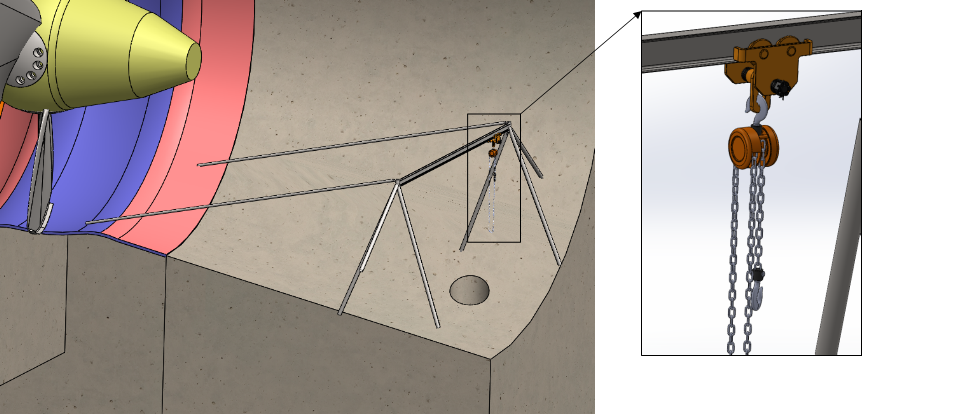
\includegraphics[width=0.8\columnwidth]{figs/bases/talha}
   \caption{Sistema de elevação dos equipamentos}
   \label{fig::talha}
\end{figure}

\begin{figure}[h!]
   \centering
   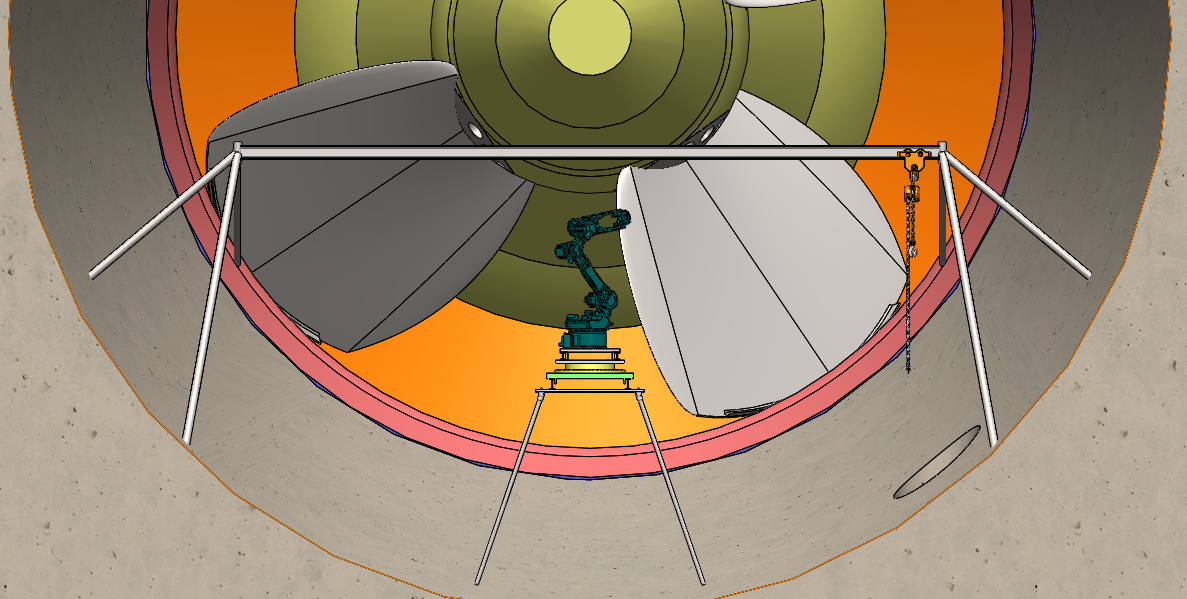
\includegraphics[width=0.8\columnwidth]{figs/bases/talha_trilho}
   \caption{Visão frontal da talha e trilho}
   \label{fig::talha_trilho}
\end{figure}

Devido aos esforços dinâmicos de operação do robô, a fixação da estutura da
base mecânica no ambiente deve ser dimensionada com cuidado. Por se
tratar de um ambiente de escoamento de fluido sob pressão, não são admitidas
modificações permanentes de infra-estrutura no interior da turbina, logo,
qualquer método de fixação utlizado deve ser removível, sem causar nenhum dano
à qualquer superfície. Em visita técnica realizada em Outrubro de $2015$ foi
testada a viabilidade de utlização de bases magnéticas para o sistema de
ancoragem e fixação. Este teste teve o objetivo de verificar a real carga limite de tração
do imã, considerando o ambiente (geometria), materiais e acabamentos
superficiais reais a que estará submetido na solução final. O resultado
detalhado do teste encontra-se no Apêndice~\ref{ape::magnetic}.

Outra opção para fixação provisória seria a soldagem da estrutura na
superfície do túnel. Esta opção segue como uma alternativa ainda para regiões
de difícil fixação da base magnética.